\PassOptionsToPackage{unicode=true}{hyperref} % options for packages loaded elsewhere
\PassOptionsToPackage{hyphens}{url}
\PassOptionsToPackage{dvipsnames,svgnames*,x11names*}{xcolor}
%
\documentclass[]{article}
\usepackage{lmodern}
\usepackage{amssymb,amsmath}
\usepackage{ifxetex,ifluatex}
\usepackage{fixltx2e} % provides \textsubscript
\ifnum 0\ifxetex 1\fi\ifluatex 1\fi=0 % if pdftex
  \usepackage[T1]{fontenc}
  \usepackage[utf8]{inputenc}
  \usepackage{textcomp} % provides euro and other symbols
\else % if luatex or xelatex
  \usepackage{unicode-math}
  \defaultfontfeatures{Ligatures=TeX,Scale=MatchLowercase}
\fi
% use upquote if available, for straight quotes in verbatim environments
\IfFileExists{upquote.sty}{\usepackage{upquote}}{}
% use microtype if available
\IfFileExists{microtype.sty}{%
\usepackage[]{microtype}
\UseMicrotypeSet[protrusion]{basicmath} % disable protrusion for tt fonts
}{}
\IfFileExists{parskip.sty}{%
\usepackage{parskip}
}{% else
\setlength{\parindent}{0pt}
\setlength{\parskip}{6pt plus 2pt minus 1pt}
}
\usepackage{xcolor}
\usepackage{hyperref}
\hypersetup{
            pdftitle={Pruebas},
            colorlinks=true,
            linkcolor=blue,
            filecolor=Maroon,
            citecolor=Blue,
            urlcolor=blue,
            breaklinks=true}
\urlstyle{same}  % don't use monospace font for urls
\usepackage[margin=1in]{geometry}
\usepackage{longtable,booktabs}
% Fix footnotes in tables (requires footnote package)
\IfFileExists{footnote.sty}{\usepackage{footnote}\makesavenoteenv{longtable}}{}
\usepackage{graphicx,grffile}
\makeatletter
\def\maxwidth{\ifdim\Gin@nat@width>\linewidth\linewidth\else\Gin@nat@width\fi}
\def\maxheight{\ifdim\Gin@nat@height>\textheight\textheight\else\Gin@nat@height\fi}
\makeatother
% Scale images if necessary, so that they will not overflow the page
% margins by default, and it is still possible to overwrite the defaults
% using explicit options in \includegraphics[width, height, ...]{}
\setkeys{Gin}{width=\maxwidth,height=\maxheight,keepaspectratio}
\usepackage[normalem]{ulem}
% avoid problems with \sout in headers with hyperref:
\pdfstringdefDisableCommands{\renewcommand{\sout}{}}
\setlength{\emergencystretch}{3em}  % prevent overfull lines
\providecommand{\tightlist}{%
  \setlength{\itemsep}{0pt}\setlength{\parskip}{0pt}}
\setcounter{secnumdepth}{5}
% Redefines (sub)paragraphs to behave more like sections
\ifx\paragraph\undefined\else
\let\oldparagraph\paragraph
\renewcommand{\paragraph}[1]{\oldparagraph{#1}\mbox{}}
\fi
\ifx\subparagraph\undefined\else
\let\oldsubparagraph\subparagraph
\renewcommand{\subparagraph}[1]{\oldsubparagraph{#1}\mbox{}}
\fi

% set default figure placement to htbp
\makeatletter
\def\fps@figure{htbp}
\makeatother


\title{Pruebas}
\author{Vásquez Guerra Carlos Fernando\\
Karyme}
\date{6/1/2020}

\begin{document}
\maketitle

{
\hypersetup{linkcolor=}
\setcounter{tocdepth}{5}
\tableofcontents
}
\hypertarget{primera-parte}{%
\section{Primera parte}\label{primera-parte}}

Hola, este es un texto de prueba \footnote{Esta es la referencia
  \(\sum_1^5\)}

Este es otro parrafo

Letras en Negritas:

\textbf{word}, \textbf{word}

Letras en cursiva:

\emph{word}, \emph{word}

\texttt{Esto\ es\ código}

20\textsuperscript{2}\textsubscript{2}

\sout{Texto tachado}

Esta es una suma \(\sum_{k=1}^nn=\frac{(n-1)(n)}{2}\).

\[
\sum_{k=1}^nn=\frac{(n-1)(n)}{2}
\]

\begin{center}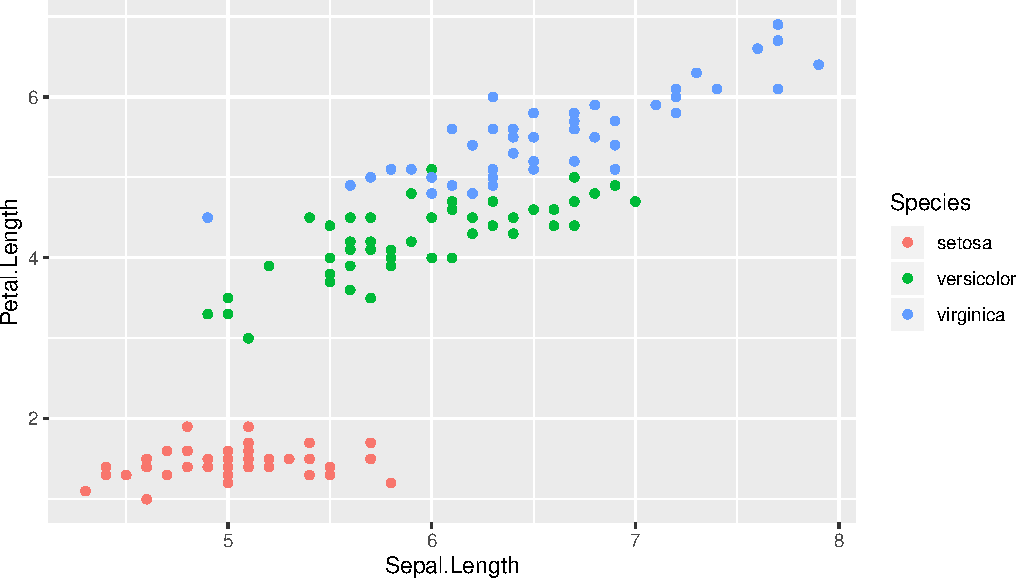
\includegraphics{Pruebas_files/figure-latex/unnamed-chunk-1-1} \end{center}

\begin{quote}
La venganza nunca es buena, mata el alma y la envenena
\end{quote}

\hypertarget{tercera}{%
\subsection{Tercera}\label{tercera}}

\begin{longtable}[]{@{}rr@{}}
\toprule
speed & dist\tabularnewline
\midrule
\endhead
4 & 2\tabularnewline
4 & 10\tabularnewline
7 & 4\tabularnewline
7 & 22\tabularnewline
8 & 16\tabularnewline
9 & 10\tabularnewline
\bottomrule
\end{longtable}

\begin{verbatim}
## [1] 30
\end{verbatim}

Aquí va el resultado 30 y ya

\hypertarget{segunda-parte}{%
\subsection{segunda parte}\label{segunda-parte}}

\href{https://es.wikipedia.org/wiki/Hoja_de_estilos_en_cascada}{CSS}

\begin{figure}
\centering

\includegraphics{keyboard-2223210_640.jpg}
\caption{Imagen}
\end{figure}

\begin{figure}
\centering

\includegraphics{Images/keyboard-2223210_640.jpg}
\caption{Imagen}
\end{figure}

\hypertarget{otro}{%
\section{Otro}\label{otro}}

\begin{figure}
\centering

\includegraphics{../Images/keyboard-2223210_640.jpg}
\caption{Imagen}
\end{figure}

\begin{itemize}
\tightlist
\item
  HOla
\item
  itme
\item
  item

  \begin{itemize}
  \tightlist
  \item
    item1.1
  \item
    item1.2
  \end{itemize}
\end{itemize}

\hypertarget{otro-subtitulo}{%
\subsubsection{Otro subtitulo}\label{otro-subtitulo}}

\begin{table}[]
\begin{tabular}{|l|l|l|l|l|}
\hline
as & as & 3 & d & 3 \\ \hline
df & fs & d & s &   \\ \hline
   &    &   &   &   \\ \hline
   &    &   &   &   \\ \hline
\end{tabular}
\end{table}

\hypertarget{otro-subitulo}{%
\paragraph{Otro subitulo}\label{otro-subitulo}}

\begin{itemize}
\tightlist
\item
  uno

  \begin{itemize}
  \tightlist
  \item
    dos -tres
  \end{itemize}
\end{itemize}

\begin{enumerate}
\def\labelenumi{\arabic{enumi}.}
\tightlist
\item
  Primero
\item
  Segundo
\item
  Tercero
\end{enumerate}

\hypertarget{otro-1}{%
\section{Otro}\label{otro-1}}

más texto

Para más información consultese \footnote{Esta es la referencia
  \(\sum_1^5\)}

\LaTeX

\end{document}
